\mainmatter%
\setcounter{page}{1}

\lectureseries[\course]{\course}

\auth[\lecAuth]{Lecturer: \lecAuth\\ Scribe: \scribe}
\date{December 1, 2009}

\setaddress%

% the following hack starts the lecture numbering at 17
\setcounter{lecture}{16}
\setcounter{chapter}{16}

\lecture{Grid-Based Numerical Methods}

\section{Grid-Based Optimization}
This is a continuation from last lecture.
The DPP is
$$V(x) = \inf_{\uinu}\left\lbrace \int_0^{\tau\wedge h}l(\xi_t,u_t)dt + I_{h<\tau}V(\xi_h) + I_{h\geq\tau}\psi(\xi_T) \right\rbrace$$
The space we are working in is
$$\mathcal{S} = \{x_{i,j}, x_{i+1,j}, x_{i-1,j}, x_{i,j+1}, x_{i,j-1}\}$$
We have the same figures as last time for the space we are working in, see Figures~\ref{fig:17grid} and~\ref{fig:17x} and note that $x_{i+1,j}-x_{i,j}=\delta$ and that $\mathcal{S}$ is a convex hull.

\begin{figure}[ht!]
\centering
\includegraphics[width=.4\textwidth]{images/16grid}
\caption{Grid for the space $G$.}
\label{fig:17grid}
\end{figure}

\begin{figure}[ht!]
\centering
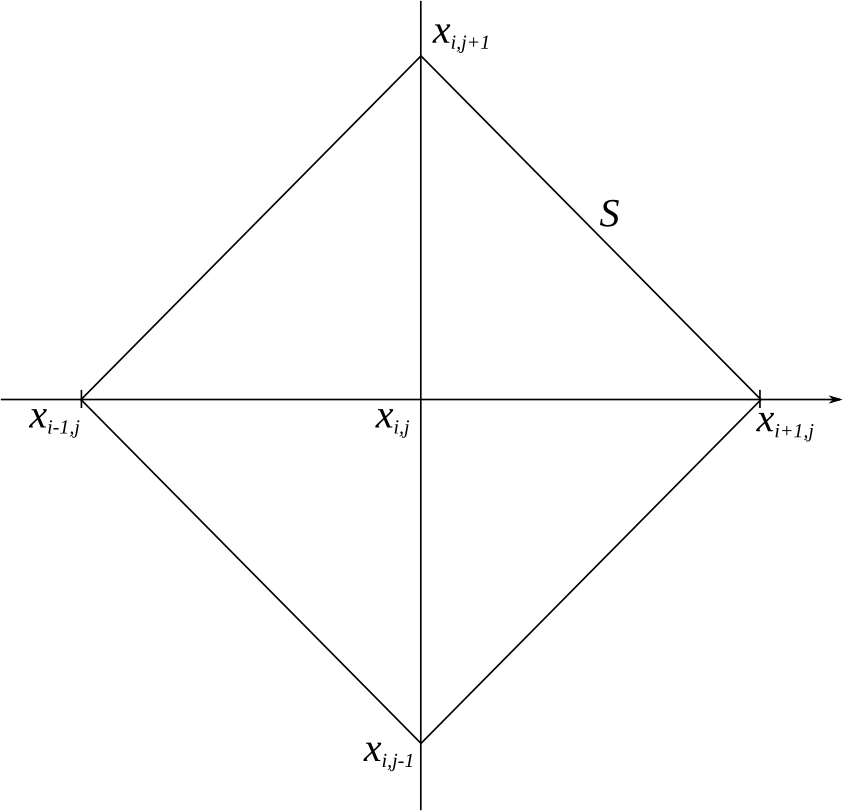
\includegraphics[width=.4\textwidth]{images/16x}
\caption{Zoomed in area around the point $x_{ij}$.}
\label{fig:17x}
\end{figure}

With $x=\xij$ we want $h$ sufficiently small such that we do not exit $G$ for any reason and that $\tau>h~\forall \epsilon$-optimal control $u$.
Then
$$V(\xij) = \inf_{u.}\left\lbrace \int_0^h l(\xi_t,u_t)dt + V(\xi_h) \right\rbrace$$
From here we do a linear approximation to get
$$V(\xij) \simeq \min_{\uinu}\left\lbrace l(\xij,u)h + V(\xij + hf(\xij,u)) \right\rbrace$$

Further suppose that $h$ is sufficiently small relative to $\delta$ such that $\xij+hf(\xij,u)\in<\mathcal{S}>$ for all reasonable controls.
Without loss of generality suppose that $\xij+hf(\xij,u)\in<\mathcal{S}_1>$ with $\mathcal{S}_1=\{\xij,x_{i+1,j},x_{i,j+1}\}$.
Then we can assume that $V$ is roughly linear in $<\mathcal{S}_1$.

Let $V^k$ be the $k$th iterate and use iteration to find
$$V^{k+1}(\xij) = \min_{\uinu}\left\lbrace l(\xij,u) + V^k(\xij+hf(\xij,u))\right\rbrace$$
if $\xij\notin\partial G$ else we have
$$V^k(\xij)=\psi(\xij)$$
if $\xij\in\partial G$.

Since $\xij+hf(\xij,u)\in\mathcal{S}_1$ we get
$$\xij+hf(\xij,u) = \lambda_1\xij + \lambda_2x_{i+1,j} + \lambda_3x_{i,j+1}$$
with
$$\lambda_1,\lambda_2,\lambda_3\in[0,1], \qquad \sum_i\lambda_i=1$$
Let
$$x_{l,m} = \left(\begin{array}{c} x_{l,m}^1 \\ x_{l,m}^2 \end{array}\right)$$
This leads to
\begin{align*}
&\lambda_1\xij^1 + \lambda_2x_{i+1,j}^1 + \lambda_3x_{i,j+1}^1 = \xij^1+hf^1(\xij,u) \\
&\lambda_1\xij^2 + \lambda_2x_{i+1,j}^2 + \lambda_3x_{i,j+1}^2 = \xij^2+hf^2(\xij,u) \\
&\lambda_1 + \lambda_2 + \lambda_3 = 1 \\
&A\vec{\lambda} = b(u) \\
\Rightarrow &\vec{\lambda} = A^{-1}b(u)
\end{align*}

Then the value function becomes
\begin{align}
\label{eq:17val}
V^{k+1}(\xij) &= \min_u\left\lbrace l(\xij,u) + V^k(\lambda_1\xij + \lambda_2x_{i+1,j} + \lambda_3x_{i,j+1}) \right\rbrace \nonumber \\
&\simeq \min_u\left\lbrace l(\xij,u)h + \lambda_1V^k(\xij) + \lambda_2V^k(x_{i+1,j}) + \lambda_3V^k(x_{i,j+1}) \right\rbrace
\end{align}
Eventually we will converge to the fixed point or vise solution.
We still need to show that this is a contraction.

\section{Max-Plus Methods}
Max-plus methods are used for deterministic control problems.
We define addition and multiplication such that
\begin{itemize}
\item $a\oplus b=\max\{a,b\}$
\item $a\otimes b = a+b$
\end{itemize}
and these hold for all $a,b\in\mathbb{R}^- = \mathbb{R}\cup\{-\infty\}$.
We can also see that
\begin{align*}
&a\oplus(-\infty) = \max\{a,-\infty\} = a~\forall a\in\mathbb{R}^- \\
&a\otimes0 = a+0=a \\
&a\otimes-a = 0
\end{align*}
where the first equation is the additive identity, the second equation is the multiplicative identity and $-a$ is the multiplicative inverse of $a$.
There is no additive inverse.

In max-plus we can have vector and function spaces such that
\begin{align*}
&\psi(x), \qquad \psi:\mathbb{R}^n\to\mathbb{R}^- \\
&[a\otimes \psi](x) = a+\psi(x) = a\otimes\psi(x)~\forall x \\
&[\psi\oplus\vp](x) = \psi(x)\oplus\vp(x) = \max\{\psi(x),\vp(x)\}~\forall x
\end{align*}

\begin{example}
\begin{align*}
\dot{\xi} &= f(\xi,u), \qquad \xi_0=x\in\mathbb{R}^n \\
J(x,T,u.) &= \int_0^T l(\xi_t,u_t)dt \\
V(x) &= \sup_{T<\infty}\sup_{u\in L_2[0,T]}J(x,T,u.)
\end{align*}
This leads to the DPP
$$V(x) = \sup_{u\in L_2[0,T]}\left\lbrace \int_0^\delta l(\xi_t,u_t)dt + V(\xi_\delta) \right\rbrace = \mathcal{S}_\delta[V](x)$$
Lets try
\begin{align*}
\mathcal{S}_\delta[c\otimes\vp](x) &= \sup_{u\in L_2}\left\lbrace \int_0^\delta l(\xi_t,u_t)dt + c\otimes\vp(\xi_\delta) \right\rbrace \\
&= c + \sup_{u\in L_2}\left\lbrace \int_0^\delta l(\xi_t,u_t)dt + \vp(\xi_\delta)\right\rbrace \\
&= c\otimes\mathcal{S}_\delta[\vp](x)
\end{align*}
$\lozenge$
\end{example}

Similarly we could show that
$$\mathcal{S}_\delta[\vp\oplus\psi](x) = \mathcal{S}_\delta[\vp](x) + \mathcal{S}_\delta[\psi](x)$$
which implies that $\mathcal{S}_\delta$ is a max-plus linear operator.

We want to solve $V=\mathcal{S}_\delta[V]$.
Recall that $0$ is the max-plus multiplicative identity and we can write
$$0\otimes V=\mathcal{S}_\delta[V]$$
This shows that $V$ is the max-plus eigenfunction corresponding the $0$.

There are two main classes of problems that max-plus methods are used to solve.
\begin{itemize}
\item Max-plus basis/max-plus finite element methods are used for complex dynamics and low dimensionality problems.
\item Max-plus curse-of-dimensionality-free methods are used for simple dynamics and high dimensionality problems.
\end{itemize}

\begin{example}
For control of quantum spin we have $u$ is the state and $V_t^m$ is the control and
\begin{align*}
&\sum_{m=1}^n{(V_t^m)}^2\leq D~\forall t \\
&\dot{U} = \left[\sum_{m=1}^n V_t^m H_m\right]U
\end{align*}
where $U\in SU(2^m)$, $U^\ast=U^{-1}$ and $|U|=1$.
If $n=2$ we are in $SU(4)$ where $SU(4)$ is equivalent to $15$-dimensional real space.
Working with $10$ grid points per dimension leads to $10^{15}$ grid points and is estimated to take $10^{12}$ hours to solve with grid points.
Max-plus methods can solve these types of problems in approximately $10$ hours!
$\lozenge$
\end{example}% chktex 17
